\documentclass[t,linespread=1.3]{ctexbeamer}

\usepackage[size=a4,orientation=portrait,scale=1.5]{beamerposter}

\usetheme{HeavenlyClouds}
% Mac 或 Linux 上请自己设定 \lishu!!
% \providecommand{\lishu}{\CJKfontspec{Libian SC}[BoldFont=Baoli SC,Scale=1.2]}
% \providecommand{\lishu}{\CJKfontspec{鸿雷板书简体-正式版.otf}[Path=fonts/]}
% 如果实在没有,就用楷书蒙混过关一下……
% \providecommand{\lishu}{\kaishu}
% 当然也可以替换别的仿宋字体,自己喜欢哈自己喜欢
% \setCJKfamilyfont{zhfs}{ZhuqueFangsong-Regular.ttf}[Path=fonts/]

\usepackage[style=gb7714-2015]{biblatex}
\addbibresource{sample-refs.bib}
\usepackage{graphicx}
\usepackage{ccicons}

% 幻灯片->海报需要的一些改动
\setbeamerfont{frametitle}{size=\Huge}
\setbeamerfont{framesubtitle}{size=\Large}
\setbeamerfont{block title}{size=\large}
\setbeamerfont{headline}{size=\small}
\setbeamerfont{footline}{size=\small}
\AddToHook{begindocument/before}{%
  \addtobeamertemplate{frametitle}{\vskip-1.5ex}{}
}

% 让神马放大一些
\setlength{\ShenmaMarkerWidth}{3.5em}
% patch for default scaling, make clouds larger 
\patchcmd{\randorn}{rnd * 0.4 + 0.1}{rnd * 0.8 + 0.3}{}{}
% patch for default opacity, make clouds more prominent on poster
\patchcmd{\randorn}{rnd * 20 + 65}{rnd * 45 + 40}{}{}
% when in portrait mode, allow clouds to be higher up
\patchcmd{\randorn}{\pgfmathsetmacro{\myy}{rnd * 0.8}}{\pgfmathsetmacro{\myy}{rnd * 0.95}}{}{}
% and further to the right too; probably more important in landscape form
\patchcmd{\randorn}{\pgfmathsetmacro{\myx}{rnd * 0.8}}{\pgfmathsetmacro{\myx}{rnd * 0.95}}{}{}
% let there be more clouds in the background
\renewcommand{\BackgroundOrns}{%
 \randorn{66}\randorn{68}\randorn{66}\randorn{70}\randorn{68}%
 \randorn{70}\randorn{68}\randorn{70}\randorn{70}%
}

\title{当神马浮云beamer主题拿来做海报}
\author{作者甲、作者乙、作者丙}

\begin{document}
\begin{frame}[fragile]
% ……简单又粗暴的,解决footline里神马的位置的方法,嗯。
\gdef\inserttotalframenumber{10}
\gdef\insertframenumber{3}

    
% ……懒得折腾了,\frametitle挺好看的,就这样吧【躺平ing
\frametitle{\insertshorttitle}
\framesubtitle{\insertshortauthor}

\begin{block}{此主题脑洞略大}

  \begin{itemize}
    \item 背景的云彩纹样,位置、大小、深浅都是随机的。刷一次不喜欢效果的话就再刷一次碰一下运气吧。
    \item 若觉得进度条上的神马太过引人注(侧)目,可以用 \verb|\simpleprogressmarker| 简单圆点取代。(默认是\verb|\shenmaprogressmarker|)。……但是这是海报啊海报,只用圆点可能真的太没存在感了。
  \end{itemize}
    
\end{block}

\begin{columns}[T]
\column{.45\textwidth}

\begin{exampleblock}{算了我也不知道在写什么,do you?}
    Now solve $x = \frac{-b \pm \sqrt{b^2 -4ac}}{2a}$. 对各位同学来说应该挑战不大。
\end{exampleblock}

\begin{alertblock}{算了我也不知道在写什么,do you?}
    \[ x = \frac{-b \pm \sqrt{b^2 -4ac}}{2a} \]
\end{alertblock}

\begin{block}{算了我也不知道在写什么,do you?}
    \[ x = \frac{-b \pm \sqrt{b^2 -4ac}}{2a} \]
\end{block}

% 个人觉得这个主题,多栏之间需要有个间隔。但是高度需要自己调整。
\column{.01\textwidth}
\textcolor{structure!80}{\rule{.1mm}{.27\textheight}}

\column{.45\textwidth}

\begin{block}{套马的汉子你威武雄壮}

  \begin{itemize}
    \item 飞驰的骏马像疾风一样
    \item 一望无际的原野随你去流浪
    \item 你的心海和大地一样宽广
  \end{itemize}

  \begin{enumerate}
      \item 你是我天边最美的云彩
      \item 让我用心把你留下来
  \end{enumerate}
\end{block}

\begin{proof}
    显而易见,$1+1=2$.
\end{proof}

\begin{theorem}
    有一件很美好的事情将要发生,它终会发生。
\end{theorem}

\end{columns}

\begin{block}{云的分类}
This is just a sample sentence with a sample citation\cite{BurroughsCrowder2007}.

\smallskip 
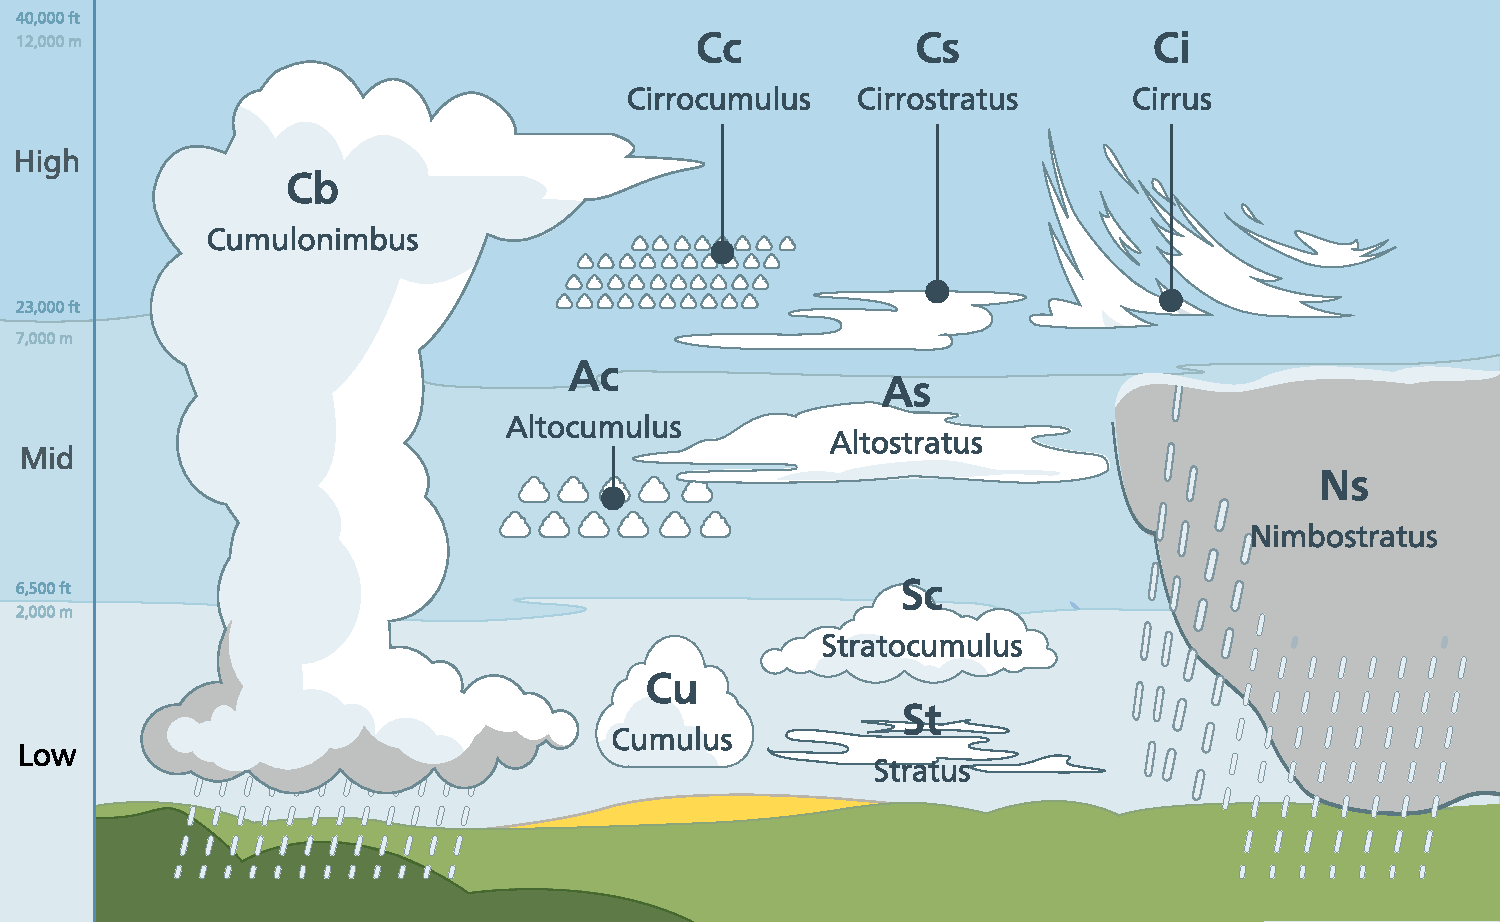
\includegraphics[width=.6\textwidth]{Cloud_types_en}\par
Valentin de Bruyn / Coton. This illustration has been created for Coton, the cloud identification guide for mobile. \ccbysa\ 3.0 via Wikimedia Commons. \url{https://commons.wikimedia.org/wiki/File:Cloud_types_en.svg}
\end{block}

\vfill

\begin{block}{\refname}
\printbibliography[heading=none]
\end{block}

\end{frame}
\end{document}
